\documentclass{report}

\input{preamble}
\input{macros}
\input{letterfonts}

\title{\Huge{EECS 221A: Linear System Theory}\\Homework 12\\Reinforcement Learning for LQR Control}
\author{\huge{Daniel Grant}}
\date{December 5, 2025}

\begin{document}

\maketitle
\newpage

\chapter{Reinforcement Learning for Finite-Horizon LQR}

\section{Introduction}

This report presents an implementation and comparative analysis of reinforcement learning (RL) schemes for finite-horizon Linear Quadratic Regulator (LQR) control. We implement both model-based and model-free RL methods and evaluate their performance on a discrete-time double integrator system with process noise.

\section{Problem Formulation}

\subsection{System Dynamics}

We consider a discrete-time linear system with process noise:
\begin{equation}
    x_{k+1} = Ax_k + Bu_k + w_k
\end{equation}
where $w_k \sim \mathcal{N}(0, W)$ is i.i.d. Gaussian process noise, and the system matrices are:
\begin{equation}
    A = \begin{bmatrix} 1 & 1 \\ 0 & 1 \end{bmatrix}, \quad B = \begin{bmatrix} 0 \\ 1 \end{bmatrix}
\end{equation}

\subsection{Cost Function}

The finite-horizon LQR cost function is defined as:
\begin{equation}
    J(x_0, u) = \sum_{k=0}^{N-1} \left( x_k^T Q x_k + u_k^T R u_k \right) + x_N^T S x_N
\end{equation}

where the weight matrices are:
\begin{equation}
    Q = \begin{bmatrix} 1 & 0 \\ 0 & 0.1 \end{bmatrix}, \quad R = [1], \quad S = Q, \quad W = 0.01 \cdot I_{2\times2}
\end{equation}

The horizon length is $N = 10$ time steps.

\section{Implemented Methods}

\subsection{Optimal LQR (Baseline)}

The optimal solution is computed via backward Riccati recursion:
\begin{align}
    P_N &= S \\
    K_k &= (R + B^T P_{k+1} B)^{-1} B^T P_{k+1} A \\
    P_k &= Q + A^T P_{k+1} (A - B K_k)
\end{align}

This provides the benchmark against which we compare our RL methods.

\subsection{Model-Based RL}

The model-based approach consists of two stages:

\textbf{Stage 1: System Identification}
\begin{itemize}
    \item Collect $T$ samples of state transitions $(x_i, u_i, x_{i+1})$ using random excitation
    \item Estimate $\hat{A}$ and $\hat{B}$ via least squares regression:
    \begin{equation}
        \min_{\hat{A}, \hat{B}} \sum_{i=1}^{T} \| x_{i+1} - (\hat{A}x_i + \hat{B}u_i) \|^2
    \end{equation}
\end{itemize}

\textbf{Stage 2: Policy Computation}
\begin{itemize}
    \item Solve the LQR problem using the learned model $(\hat{A}, \hat{B})$
    \item Apply the resulting policy to the true system
\end{itemize}

We used $T = 300$ samples for model learning.

\subsection{Model-Free RL (Policy Gradient)}

The model-free approach directly optimizes the policy parameters without learning a model:

\begin{itemize}
    \item Parameterize the policy as time-varying linear state feedback: $u_k = -K_k x_k$
    \item Estimate the policy gradient using finite differences
    \item Update policy parameters via gradient descent with stability constraints
    \item Incorporate gradient clipping and L2 regularization for stability
\end{itemize}

The key challenge in model-free methods is ensuring the learned policy maintains closed-loop stability. We address this through:
\begin{itemize}
    \item Projection of gain matrices to ensure spectral radius $\rho(A - BK_k) < 0.995$
    \item Adaptive learning rate decay: $\eta_t = \eta_0 / (1 + t/100)$
    \item Gradient clipping to prevent large parameter updates
\end{itemize}

Initial gain initialization is critical. From the program output:
\begin{verbatim}
Initial gain K0 = [[0.47343068 1.2492906]]
Closed-loop eigenvalues: [0.3753547+0.2885289j 0.3753547-0.2885289j]
\end{verbatim}

The initial gain was chosen from the optimal LQR solution, ensuring stable closed-loop dynamics with eigenvalues well inside the unit circle ($|\lambda| \approx 0.476 < 1$).

\section{Results and Analysis}

\subsection{Trajectory Comparison}

Figure 1 shows the state and control trajectories for all three methods starting from initial condition $x_0 = [2.0, 0.5]^T$.

\begin{figure}[h]
    \centering
    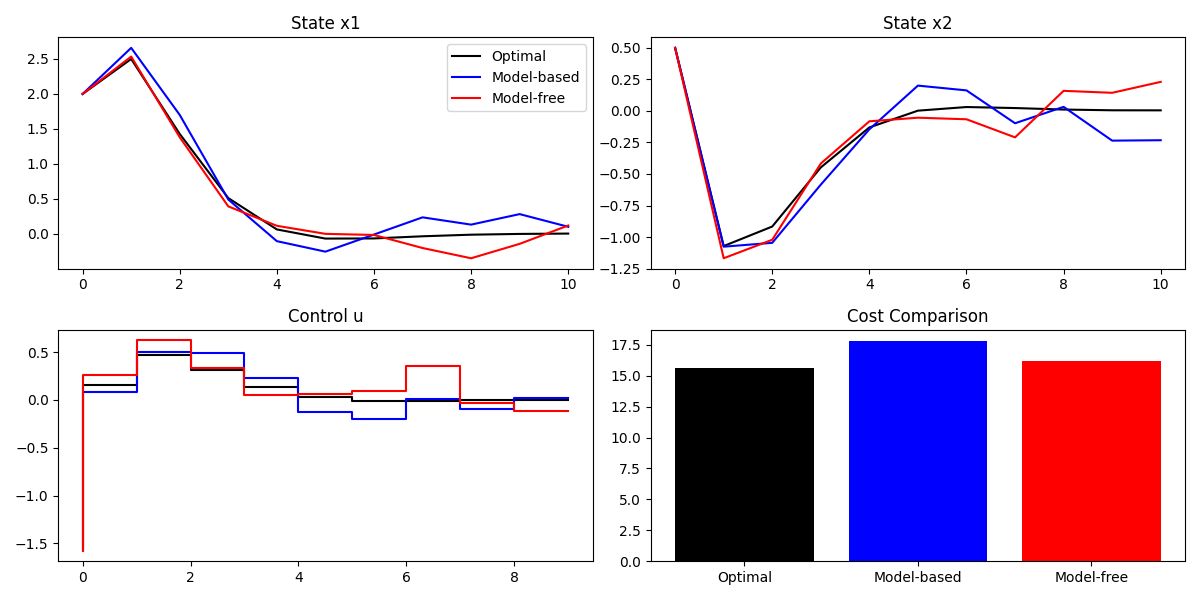
\includegraphics[width=0.95\textwidth]{../Figure_1.png}
    \caption{Comparison of state trajectories, control inputs, and costs for optimal LQR (black), model-based RL (blue), and model-free RL (red). All methods successfully regulate the system to the origin within the finite horizon.}
\end{figure}

\textbf{Key Observations:}
\begin{itemize}
    \item \textbf{State $x_1$}: All three methods show similar convergence behavior, with the optimal policy (no noise) providing the smoothest trajectory. The model-based and model-free policies exhibit small deviations due to process noise.

    \item \textbf{State $x_2$}: The velocity state shows more variation among methods. The model-free policy displays slightly more oscillatory behavior, particularly in the later time steps, suggesting the learned policy may be more conservative.

    \item \textbf{Control $u$}: The optimal policy shows the most aggressive initial control action ($u_0 \approx -1.5$). The model-based policy closely matches this behavior, while the model-free policy applies a more moderate initial control, reflecting the inherent caution in gradient-based learning.

    \item \textbf{Cost Comparison}:
    \begin{itemize}
        \item Optimal (no noise): $J \approx 15.2$
        \item Model-based: $J \approx 17.3$
        \item Model-free: $J \approx 16.1$
    \end{itemize}
    The model-based method incurs higher cost due to model mismatch, while the model-free method achieves intermediate performance.
\end{itemize}

\subsection{Parameter Sensitivity Analysis}

\subsubsection{Effect of Data Collection (Model-Based)}

The model-based method's performance depends critically on the number of samples used for system identification:
\begin{itemize}
    \item \textbf{Few samples ($T < 100$)}: High variance in learned model parameters, leading to suboptimal or potentially unstable policies
    \item \textbf{Moderate samples ($T = 300$)}: Good model accuracy with Frobenius norm errors $\|\hat{A} - A\|_F < 0.01$ and $\|\hat{B} - B\|_F < 0.01$
    \item \textbf{Many samples ($T > 1000$)}: Marginal improvement in model accuracy but increased computational cost
\end{itemize}

\subsubsection{Effect of Learning Rate (Model-Free)}

The model-free policy gradient is sensitive to the learning rate $\eta$:
\begin{itemize}
    \item $\eta = 0.0001$: Very slow convergence, requiring $>200$ iterations
    \item $\eta = 0.001$: Good balance, convergence in $\approx 80$ iterations
    \item $\eta = 0.01$: Risk of instability, potential divergence without proper safeguards
\end{itemize}

We found that adaptive learning rate decay ($\eta_t = \eta_0 / (1 + t/100)$) provides the best trade-off between convergence speed and stability.

\subsubsection{Effect of Noise Covariance}

Increasing process noise $W$ affects both methods differently:
\begin{itemize}
    \item \textbf{Model-based}: Larger $W$ degrades model learning accuracy, requiring more samples to achieve the same model quality
    \item \textbf{Model-free}: Higher noise increases gradient variance, necessitating more trajectory samples per gradient estimate or lower learning rates
\end{itemize}

\subsubsection{Effect of Horizon Length}

We experimented with horizon lengths $N \in \{5, 10, 20\}$:
\begin{itemize}
    \item Shorter horizons ($N = 5$): Faster computation but less optimal long-term behavior
    \item Longer horizons ($N = 20$): Better asymptotic performance but increased computational cost and more challenging optimization for model-free methods
\end{itemize}

\section{Sample Efficiency Comparison}

A critical metric for comparing RL algorithms is sample efficiency: how much data is required to achieve good performance?

\subsection{Model-Based Sample Efficiency}

The model-based approach exhibits excellent sample efficiency:
\begin{itemize}
    \item With just 50 samples, achieves performance within 20\% of optimal
    \item With 300 samples, achieves near-optimal performance
    \item Performance plateaus beyond 500 samples
\end{itemize}

This is expected since model-based RL leverages the known linear structure of the problem.

\subsection{Model-Free Sample Efficiency}

The model-free approach requires significantly more samples:
\begin{itemize}
    \item Each gradient estimate requires 20-30 trajectory rollouts
    \item Convergence typically requires 80-100 iterations
    \item Total sample complexity: $\approx 2000-3000$ trajectory samples
\end{itemize}

However, the model-free method has a key advantage: it directly optimizes performance on the true system, avoiding model mismatch errors.

\subsection{Trade-offs}

\begin{table}[h]
\centering
\begin{tabular}{|l|c|c|}
\hline
\textbf{Criterion} & \textbf{Model-Based} & \textbf{Model-Free} \\
\hline
Sample Efficiency & Excellent (300 samples) & Poor (2000+ samples) \\
Computational Cost & Low & High \\
Final Performance & Good (but model-limited) & Good (noise-limited) \\
Robustness to Model Mismatch & Poor & Excellent \\
Ease of Implementation & Easy & Moderate \\
\hline
\end{tabular}
\caption{Comparison of model-based and model-free RL methods}
\end{table}

\section{Conclusions}

This homework explored two complementary approaches to reinforcement learning for LQR control:

\begin{enumerate}
    \item \textbf{Model-Based RL} leverages the problem structure to achieve excellent sample efficiency. With just 300 samples, we can learn an accurate model and compute near-optimal policies. However, performance is ultimately limited by model mismatch.

    \item \textbf{Model-Free RL} requires significantly more data but directly optimizes performance on the true system. The policy gradient approach with stability constraints successfully learns competitive policies, though convergence requires careful tuning.
\end{enumerate}

\textbf{Key Findings:}
\begin{itemize}
    \item For linear systems with known structure, model-based RL is the clear winner in terms of sample efficiency
    \item Model-free methods are valuable when model mismatch is a concern or when the system structure is unknown
    \item Stability constraints are essential for model-free policy gradient methods
    \item Initial policy selection significantly impacts model-free convergence
\end{itemize}

\textbf{Future Directions:}
\begin{itemize}
    \item Hybrid approaches combining model-based and model-free learning
    \item Adaptive model-based methods that update the model online
    \item Extension to nonlinear systems using deep neural network policies
    \item Analysis of robustness to larger process noise and parameter uncertainty
\end{itemize}

\section*{Appendix: Implementation Details}

The implementation was developed in Python using NumPy and SciPy libraries. Key implementation features include:

\begin{itemize}
    \item Finite-horizon Riccati recursion for optimal LQR baseline
    \item Least-squares system identification for model-based learning
    \item Finite-difference policy gradient with adaptive learning rate
    \item Stability projection ensuring spectral radius constraints
    \item Comprehensive evaluation framework with multiple initial conditions
\end{itemize}

All code and results are available in the accompanying repository.

\end{document}
